% -*- root: ../thesis.tex -*-
%%%%%%%%%%%%%%%%%%%%----------%%%%%%%%%%%%%%%%%%%%
%%%
% 	Author: Boris Kourtoukov
%   Project: Digital Futures Thesis Document
%   Title: Periphery
% 	File: Narrative
%%%
%%%%%%%%%%%%--------------------------%%%%%%%%%%%%

\mqp{What comprises Periphery?}
Through the work on this project Periphery has been distilled into three clear parts: 

\begin{itemize}
  \item Stable and wearable ambient sensor network.
  \item Application Porogramming Interface (API) for the collected data.
  \item Visual style guide for future wearables.
\end{itemize}

\newthought{This chapter will} focus on the visual style guide. It was created with the support from Chenthooran Nambiarooran\sidenote{\url{http://chenthooran.com/}}, he is concept artist and illustrator based out of London.

\section{Design Inspiration}

\mqp{What influenced the development of the style guide?}
The primary inspiration for the art exploration in the project was cyberpunk literature, film, and games. Authors like William Gibson\sidenote{\url{http://www.williamgibsonbooks.com/}} and Neal Stephenson\sidenote{\url{http://www.nealstephenson.com/}} created a very intriguing depictions of what the technology of our near future would be like. Films include Johnny Mnemonic\sidenote{\url{http://www.imdb.com/title/tt0113481/}} and Blade Runner\sidenote{\url{http://bladerunnerthemovie.warnerbros.com/}} and provided a deeper visual exploration of what has become a very iconic style. While Deus Ex\sidenote{\url{http://www.deusex.com/}} explored the minutiae of this setting in much greater quantities through the need of a vast variety of in-game assets. The main problem that arises from this media is the focus on the violent uses of technology. This creates a mixture of pleasing aesthetics with a clear threatening tone. The Periphery style guide strives to focus entirely on the pleasing aspects of this media, and forgo the harsher elements.
\FloatBarrier

\section{Design Constraints}\label{sec:designconstraints}

It is important to keep in mind that this is a modern day device. Although the aesthetics will be deeply rooted in a great deal of our current sci-fi and cyberpunk art the final outcome needs to function outdoors today.

Sketches should have at least some inspiration from the everyday and mundane. As some examples:

\begin{itemize}
  \item Public transit
  \item Restaurants
  \item Rain
  \item Running
  \item Bumping into things
  \item Coming into physical contact with others
\end{itemize}

To elaborate, if I end up hugging someone it shouldn’t end in blood. If I trip I shouldn’t have chunks of plastic everywhere. Although the latter is upto my material exploration and not so much the concept art it is still something that can influence the shape.
Outcomes

The main outcome that needs to come from the concept artwork for this thesis is a set of reusable, modular and visually striking elements. These elements include:

\begin{itemize}
  \item Textures and patterns
  \item Key shapes
  \item The colour scheme
  \item Repeaters and Rhythm
\end{itemize}

The last being something akin to `wool before acrylic but only after solid gold', repeatable material/shape patterns that can become immediate areas of recognition. (The `oh yeah thats a piece of that project!')

The illustrations shown are not intended as blueprints for the final physical result. Instead, they represent various stages of thought reflecting the iterative design process that is informing my development process.
General Notes

The following few points are some general constraints. These are intended to say what this project won’t have in the end and not what shouldn’t be considered during this stage.

\begin{itemize}
  \item Nothing that covers the face. (I am not planning to tackle that area of wearable tech, and there are plenty of projects that can already be worn on one’s head to compliment the final outcome.)
  \item Nothing on the feet. (From an early stage I realized what kind of nightmare it would be to prototype something in a short time that will stay intact on ones feet)
  \item Generally placing things above the waist.
\end{itemize}

Again these are for ease of development, and the artwork can go into these areas as long as it helps further the general reusable and repeatable patterns and ideas.
A note about the sources of inspiration:

As a great deal of artwork that exists today in the sci-fi and cyberpunk genres is of military, violent or menacing nature it is one of the challenges in this project to extract the aspects that make that art inspiring while detaching these negative connotations.

To put together the main goals of this concept art stage:

\begin{quote}
The outcome should be a visually inspiring, modular and practical (but only to the extent of not constricting movement and damaging innocent bystanders) set of wearables on the body.
\end{quote}

\section{The Concepts}

\begin{figure}
  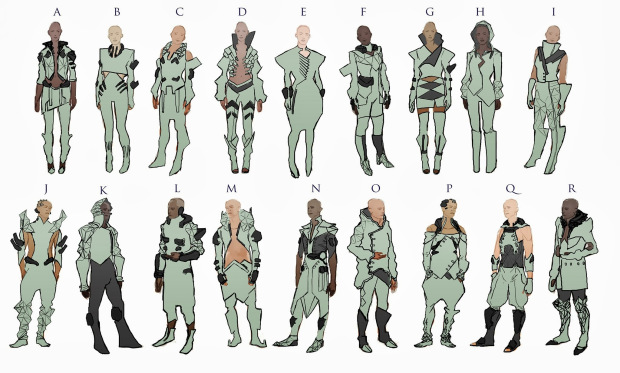
\includegraphics{clotherie1.jpg}
  \caption{Results from the second round and a set of more dynamic poses. A piece from the preliminary sketches below.}
  \label{fig:secondround}
\end{figure}

\begin{marginfigure}
  \includegraphics[scale=0.5]{figure3.png}
  %\caption{Part of preliminary sketches.}
  \label{fig:secondround}
\end{marginfigure}

Following the constraints and inspiration mentioned above, Chenthooran created a number of iterations that reflected in a final set of modules. The positions of modules were not determined from the start, although they were influenced by the ``Design for Wearability'' paper \citep{Gemperle98} described earlier. The final modules settled on the upper arms, hip, and neck. During this phase, the design has been intentionally left without the influence of physical electronic restrictions, thus allowing for a more reusable final style guide.

\begin{figure}
  \includegraphics[scale=0.5]{other_poses.jpg}
  \caption{More dynamic poses.}
  \label{fig:dynamicposes}
\end{figure}

\begin{figure}
  \includegraphics{modules1.jpg}
  \caption{Closer subset of modules.}
  \label{fig:subsetofmods}
\end{figure}

\begin{figure}
  \includegraphics{modules2v2.jpg}
  \caption{Three selected module shapes.}
  \label{fig:selectedmods}
\end{figure}

\begin{figure*}
  \includegraphics{modules3fixed2.jpg}
  \caption{A closer detail of the final shapes.}
  \label{fig:finalmods}
\end{figure*}
